\section{Perceptron Model}
\label{pmodel}

\subsection{Artificial Neural Networks}

The Hebbian Theory allows a computer to distinguish similarities in the features between inputs. This is because, over time, a \gls{neuron} that represents a feature will be associated with that feature in the input. However, we do not know what these features are, only that they are common within inputs. We, therefore, need another \gls{model} that takes these \gls{neuron}s and decides what the features represent. For this to work, we need a desired output for each input, telling the \gls{model} which features are important to which input, to determine the correct output.
This is what the \gls{perceptron} \gls{model} attempts to do.

\subsubsection{Neuron Model}

Consider a \gls{neuron} $y$. There are many \gls{neuron}s connected to $y$, $x_1, x_2, \cdots, x_I$. The \gls{axon} from $x_i$, $\text{A}(x_i)$, is connected to the $i^\text{th}$ \gls{dend} of $y$, $\text{D}_i(y)$, via a weighted \gls{synapse} $w_{i}$. Therefore $\text{D}_i(y)=w_i\text{A}(x_i)$. The \gls{dend}s of $y$ are combined to give the \gls{axon} of $y$, $\text{A}(y)$.\cite[p.~84]{nnd}

The \gls{axon} of $y$ can be simply \gls{model}led as 
\begin{equation}
\begin{split}
    \text{A}(y)&=\sum^I_{i=1}\text{D}_i(y)\\
    &=\sum^I_{i=1}w_i\text{A}(x_i)
\end{split}
\label{eq:nnmaxon}
\end{equation} 

If the \gls{axon} of $x_i$ is deactivated, $x_i=0$, the \gls{dend} of $x_i$ will always be zero, thus losing information. We must therefore add a bias, so our function does not need to be proportional.

\begin{equation}
\begin{split}
    \text{A}(y)=b+\sum^I_{i=1}w_i\text{A}(x_i)
\end{split}
\label{eq:nmaxon}
\end{equation} 

Since we are dealing with just the \gls{axon}s of $x_i$ and $y$, we can simplify \eq{eq:nmaxon} as 
\begin{equation}
y=b+\sum^I_{i=1}w_ix_i
\label{eq:nmsimple}
\end{equation}


\subsubsection{Network Architecture}

$x_i$ and $y$ are \gls{neuron}s, which can be \gls{model}ed as nodes

\begin{figure}[ht]
\setlength{\unitlength}{0.14in} % selecting unit length
\centering % used for centering Figure
\begin{picture}(10,5) % picture environment with the size (dimensions)
 % 32 length units wide, and 15 units high.
\put(0.8, 0){$\vdots$}
\put(-0.1, 1.6){\framebox(2.2, 2.2){$x_i$}}
\put(0.8, 4.4){$\vdots$}

\put(7.9, 1.6){\framebox(2.2, 2.2){$y$}}

\end{picture}
\caption{\gls{model} of $x$ \gls{neuron}s and $y$ \gls{neuron}}
\label{fig:xiy} 
\end{figure}

These \gls{neuron}s are connected via \gls{synapse}s, which can be \gls{model}ed as a line connecting the \gls{neuron}s.

\begin{figure}[ht]
\setlength{\unitlength}{0.14in}
\centering
\begin{picture}(10,5)


\put(0.8, 0){$\vdots$}
\put(-0.1, 1.6){\framebox(2.2, 2.2){$x_i$}}
\put(0.8, 4.4){$\vdots$}

\put(7.9, 1.6){\framebox(2.2, 2.2){$y$}}

\mline{1.5}{0.5}{6.0}{2.15}\mline{2.5}{2.65}{5.0}{0.0}\mline{1.5}{4.8}{6.0}{-2.15}

\end{picture}
\caption{\gls{model} of $x$ \gls{neuron}s connected to $y$ \gls{neuron} with \gls{synapse}s}
\label{fig:xiys}
\end{figure}

We can add more \gls{neuron}s, $y_j$, from the same input \gls{neuron}s, $x_i$, using different \gls{synapse}s. This will increase the complexity of the neural network, allowing for more flexibility.

\begin{figure}[H]
\setlength{\unitlength}{0.14in}
\centering
\begin{picture}(10,5) 
\put(0.8, 0){$\vdots$}
\put(-0.1, 1.6){\framebox(2.2, 2.2){$x_i$}}
\put(0.8, 4.4){$\vdots$}

\put(8.8, 0){$\vdots$}
\put(7.9, 1.6){\framebox(2.2, 2.2){$y_j$}}
\put(8.8, 4.4){$\vdots$}

\mline{1.5}{0.5}{7.0}{0.0}
\mline{1.5}{0.5}{6.0}{2.15}
\mline{1.5}{0.5}{7.0}{4.3}

\mline{2.5}{2.65}{6.0}{2.15}
\mline{2.5}{2.65}{5.0}{0.0}
\mline{2.5}{2.65}{6.0}{-2.15}

\mline{1.5}{4.8}{7.0}{-4.3}
\mline{1.5}{4.8}{6.0}{-2.15}
\mline{1.5}{4.8}{7.0}{0.0}

\end{picture}
\caption{\gls{model} of $x$ \gls{neuron}s to $y$ \gls{neuron}s with \gls{synapse}s}
\label{fig:xiyjs}
\end{figure}

In a neural network, there are input, \gls{hidden}, and output \gls{layer}s, where a \gls{layer} contains \gls{neuron}s that activate at the same time at a specific depth within the network. \cite[p.~87]{nnd}

\begin{figure}[H]
\setlength{\unitlength}{0.14in}
\centering
\begin{picture}(34,5) 

\put(0.8, 0){$\vdots$}
\put(-0.1, 1.6){\framebox(2.2, 2.2){$x_i$}}
\put(0.8, 4.4){$\vdots$}

\put(8.4, 0){\reflectbox{$\ddots$}}
\put(8.4, 2.4){$\cdots$}
\put(8.4, 4.4){$\ddots$}

\put(16.8, 0){$\vdots$}
\put(15.9, 1.6){\framebox(2.2, 2.2){$h^L_n$}}
\put(16.8, 4.4){$\vdots$}

\put(24.4, 0){$\ddots$}
\put(24.4, 2.4){$\cdots$}
\put(24.4, 4.4){\reflectbox{$\ddots$}}

\put(32.8, 0){$\vdots$}
\put(31.9, 1.6){\framebox(2.2, 2.2){$y_j$}}
\put(32.8, 4.4){$\vdots$}

\mline{1.5}{0.5}{6.4}{0.0}
\mline{1.5}{0.5}{6.4}{2.15}
\mline{1.5}{0.5}{6.4}{4.3}

\mline{2.5}{2.65}{5.4}{2.15}
\mline{2.5}{2.65}{5.4}{0.0}
\mline{2.5}{2.65}{5.4}{-2.15}

\mline{1.5}{4.8}{6.4}{-4.3}
\mline{1.5}{4.8}{6.4}{-2.15}
\mline{1.5}{4.8}{6.4}{0.0}


\mline{10.1}{0.5}{6.4}{0.0}
\mline{10.1}{0.5}{5.4}{2.15}
\mline{10.1}{0.5}{6.4}{4.3}

\mline{10.1}{2.65}{6.4}{2.15}
\mline{10.1}{2.65}{5.4}{0.0}
\mline{10.1}{2.65}{6.4}{-2.15}

\mline{10.1}{4.8}{6.4}{-4.3}
\mline{10.1}{4.8}{5.4}{-2.15}
\mline{10.1}{4.8}{6.4}{0.0}


\mline{17.5}{0.5}{6.4}{0.0}
\mline{17.5}{0.5}{6.4}{2.15}
\mline{17.5}{0.5}{6.4}{4.3}

\mline{18.5}{2.65}{5.4}{2.15}
\mline{18.5}{2.65}{5.4}{0.0}
\mline{18.5}{2.65}{5.4}{-2.15}

\mline{17.5}{4.8}{6.4}{-4.3}
\mline{17.5}{4.8}{6.4}{-2.15}
\mline{17.5}{4.8}{6.4}{0.0}


\mline{26.1}{0.5}{6.4}{0.0}
\mline{26.1}{0.5}{5.4}{2.15}
\mline{26.1}{0.5}{6.4}{4.3}

\mline{26.1}{2.65}{6.4}{2.15}
\mline{26.1}{2.65}{5.4}{0.0}
\mline{26.1}{2.65}{6.4}{-2.15}

\mline{26.1}{4.8}{6.4}{-4.3}
\mline{26.1}{4.8}{5.4}{-2.15}
\mline{26.1}{4.8}{6.4}{0.0}


\end{picture}
\caption{\gls{model} of $x$ input \gls{neuron}s connected to $h^L$ \gls{neuron}s connected to $y$ output \gls{neuron}s}
\label{fig:xihLnyj}
\end{figure}

More \gls{layer}s allow for more complex functions. We will discuss how to correctly determine the complexity in \sect{params}, and we will discuss the implications of not using this method in \sect{lim}.

\subsection{Gradient Descent}

So far we have discussed how information is propagated forward through the network to produce an output, however, there is no way we can change the weights of each \gls{synapse} to achieve a different output, and thus learn.

Gradient Descent attempts to minimise the \gls{cost}, $\nabla C$, of a neural network, which is a measure of how well it maps the target data. There are many ways of doing this, but for our simple feedforward architecture, the most common method is backpropagation.

\subsubsection{Backpropagation}
\label{backprop}
Backpropagation aims to change the weights of a neural network in the most efficient way such that the output of the neural network fits closer to the desired output, given a specified input. 

Consider the following neural network.

\begin{figure}[ht]
\setlength{\unitlength}{0.14in}
\centering
\begin{picture}(13.1,5) 
\put(10.3, 0.8){$b$}
\put(9.6, 0.9){\framebox(0.5, 0.5){}}
\put(-0.1, 1.6){\framebox(2.2, 2.2){$X$}}
\put(4.6, 3){$w$}
\put(7.9, 1.6){\framebox(2.2, 2.2){$O$}}
\put(10.9, 1.6){\framebox(2.2, 2.2){$Y$}}

\mline{2.5}{2.65}{5.0}{0.0}

\end{picture}
\caption{\gls{model} of \gls{neuron} $X$ connected to \gls{neuron} $O$ with a weighted \gls{synapse} $w$}
\label{fig:XwO}
\end{figure}

We can describe the how close the output, $O$, is to the target, $Y$, with the \gls{cost}, $C$, which is equal to the square of the difference of $O$ and $Y$. We square this value so that the \gls{cost} is positive, and it is continuously differentiable, which will prove very useful later on.\cite[p.~313]{nnd} $$C=(O-Y)^2$$

We can make a graph of how $w$ affects $C$, so we can find what weight gives the minimum \gls{cost}, and therefore the closest output to our target. 

\begin{figure}[ht]
\setlength{\unitlength}{0.14in}
\centering
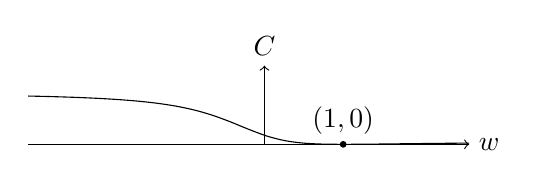
\begin{tikzpicture}
\draw[->] (-3,0) -- (2.6,0) node[right] {$w$};
\draw[->] (0,0) -- (0,1) node[above] {$C$};
\draw[scale=1.0,domain=-3:2.6,smooth,variable=\x,black] plot ({\x},{(((1/(1+e^(-(\x*-3))))-(1/(1+e^(-(-3)))))^2+((1/(1+e^(-(\x*-2))))-(1/(1+e^(-(-2)))))^2+((1/(1+e^(-(\x*-1))))-(1/(1+e^(-(-1)))))^2+((1/(1+e^(-(\x*0))))-(1/(1+e^(-(0)))))^2+((1/(1+e^(-(\x*1))))-(1/(1+e^(-(1)))))^2+((1/(1+e^(-(\x*2))))-(1/(1+e^(-(2)))))^2+((1/(1+e^(-(\x*3))))-(1/(1+e^(-(3)))))^2)/7});
\filldraw[black] (1,0) circle (1pt) node[anchor=south] {$(1,0)$};
\end{tikzpicture}
\caption{A graph of $C$ against $w$}
\label{fig:Cw}
\end{figure}

We know that where $w=1$, we achieve a \gls{cost} of $0$, so the output is equal to the input. However, we do not want to iterate through all possible weights in a neural network to find the minimum \gls{cost}, as that is very computationally expensive. Instead, we should start at a random $w$, say $-1$, and take small steps downhill, hence gradient descent. 

\begin{figure}[ht]
\setlength{\unitlength}{0.14in}
\centering
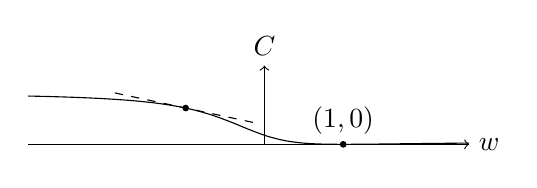
\begin{tikzpicture}
\draw[->] (-3,0) -- (2.6,0) node[right] {$w$};
\draw[->] (0,0) -- (0,1) node[above] {$C$};
\draw[scale=1.0,domain=-3:2.6,smooth,variable=\x,black] plot({\x},{(((1/(1+e^(-(\x*-3))))-(1/(1+e^(-(-3)))))^2+((1/(1+e^(-(\x*-2))))-(1/(1+e^(-(-2)))))^2+((1/(1+e^(-(\x*-1))))-(1/(1+e^(-(-1)))))^2+((1/(1+e^(-(\x*0))))-(1/(1+e^(-(0)))))^2+((1/(1+e^(-(\x*1))))-(1/(1+e^(-(1)))))^2+((1/(1+e^(-(\x*2))))-(1/(1+e^(-(2)))))^2+((1/(1+e^(-(\x*3))))-(1/(1+e^(-(3)))))^2)/7});
\draw[scale=1.0,domain=-1.9:-0.1,dashed,variable=\x,black] plot({\x},{-0.21340427*\x+0.46082-0.21340427});
\filldraw[black] (1,0) circle (1pt) node[anchor=south] {$(1,0)$};
\filldraw[black] (-1,0.46082) circle (1pt);
\end{tikzpicture}
\caption{A graph of $C$ against $w$ showing the gradient at $w=-1$}
\label{fig:Cwm}
\end{figure}
We can decrease the \gls{cost}, $C$, by repeatedly changing $w$ proportionally to the negative gradient at $w$, or 
\begin{equation}
\Delta w=-\alpha\frac{\partial C}{\partial w}
\end{equation}
where $\alpha$ is the learning rate, which is essentially how big of a step in the given direction you take - too small, and it will take too long finding the minima - too large, and you will overshoot the minima, almost rocking back and forth. 

Now, all we need to do is find the gradient.

\subsubsection{Using the Chain Rule}
\label{chain}

Using \fig{fig:XwO}, we can express $C$ using the following functions 
\begin{equation}
\begin{split}
&C=(O-Y)^2\\
&O=\sigma(z)\\
&z=wX+b
\end{split}
\end{equation}
Using the chain rule, we can equate
\begin{equation}
\begin{split}
\frac{\partial C}{\partial w}&=\frac{\partial C}{\partial O}\frac{\partial O}{\partial z}\frac{\partial z}{\partial w}\\
&=2(O-Y)\sigma'(z)X
\label{eq:crw}
\end{split}
\end{equation}
\eq{eq:crw} only works for \fig{fig:XwO}, so we need a more general \gls{model}.

It is important to take notice of the function $\sigma()$. This is what is known as the \gls{activation} function, and limits the range of the value of a neuron. In this example, and everywhere else in this dissertation, we use the activation function sigmoid, and its range is denoted as $0<\sigma(x)<1$.

Since we are dealing with multiple \gls{neuron}s, weights, and \gls{layer}s, we need a syntax to index these:

$x^L_i$ represents the $i^\text{th}$ \gls{neuron} in \gls{layer} $L$;
$Y^L_i$ represents the target for $x^L_i$;
$n_L$ represents the number of \gls{neuron}s in \gls{layer} $L$;
$w^L_{ij}$ represents the weight of the \gls{synapse} connected to the $i^\text{th}$ \gls{neuron} in \gls{layer} $L$, from the $j^\text{th}$ \gls{neuron} in \gls{layer} $L-1$. 

Consider \fig{fig:targetnet}

\begin{figure}[ht]
\setlength{\unitlength}{0.14in}
\centering
\begin{picture}(16,5) 

\put(0.8, 0){$\vdots$}
\put(-0.1, 1.6){\framebox(2.2, 2.2){$Y^{L-1}_k$}}
\put(0.8, 4.4){$\vdots$}

\put(3.8, 0){$\vdots$}
\put(2.9, 1.6){\framebox(2.2, 2.2){$x^{L-1}_k$}}
\put(3.8, 4.4){$\vdots$}

\put(2.9, 0.9){\framebox(0.5, 0.5){}}
\put(12.6, 0.9){\framebox(0.5, 0.5){}}

\put(11.8, 0){$\vdots$}
\put(10.9, 1.6){\framebox(2.2, 2.2){$x^{L}_j$}}
\put(11.8, 4.4){$\vdots$}

\put(14.8, 0){$\vdots$}
\put(13.9, 1.6){\framebox(2.2, 2.2){$Y^{L}_j$}}
\put(14.8, 4.4){$\vdots$}

\mline{4.5}{0.5}{7.0}{0.0}
\mline{4.5}{0.5}{6.0}{2.15}
\mline{4.5}{0.5}{7.0}{4.3}

\mline{5.5}{2.65}{6.0}{2.15}
\mline{5.5}{2.65}{5.0}{0.0}
\mline{5.5}{2.65}{6.0}{-2.15}

\mline{4.5}{4.8}{7.0}{-4.3}
\mline{4.5}{4.8}{6.0}{-2.15}
\mline{4.5}{4.8}{7.0}{0.0}

\end{picture}
\caption{\gls{model} of \gls{neuron}s $x^{L-1}$ in \gls{layer} $L-1$ with targets $Y^{L-1}$ connected to \gls{neuron}s $x^L$ in \gls{layer} $L$ with targets $Y^L$.}
\label{fig:targetnet}
\end{figure}
The \gls{cost} from multiple outputs is the sum of each \gls{cost} of the output to the corresponding output.
\begin{equation}
\begin{split}
&C=\sum_{j=0}^{n_L-1}{(x^L_j-Y^L_j)^2}\\
&x^L_j=\sigma(z^L_j)\\ 
&z^L_j=b^L_j+\sum_{k=0}^{n_{L-1}-1}w_{jk}^Lx_{k}^{L-1}    
\end{split}
\end{equation}


We can reevaluate the gradient again using the chain rule.

\begin{equation}
\begin{split}
\Delta w_{jk}^L&=-\alpha\frac{\partial C}{\partial w_{jk}^L}\\
\frac{\partial C}{\partial w_{jk}^L}&=\frac{\partial C}{\partial x^L_j}\frac{\partial x^L_j}{\partial z^L_j}\frac{\partial z^L_j}{\partial w_{jk}^L}\\
&=2(x_{j}^{L}-Y^L_j)\sigma'(z^L_j)x^{L-1}_k
\end{split}
\label{eq:gcrw}
\end{equation}

To find out what $b^L_j$ should be we can use the chain rule against $b^L_j$.

\begin{equation}
\begin{split}
\Delta b^L_j&=-\alpha\frac{\partial C}{\partial b^L_j}\\
\frac{\partial C}{\partial b^L_j}&=\frac{\partial C}{\partial x^L_j}\frac{\partial x^L_j}{\partial z^L_j}\frac{\partial z^L_j}{\partial b^L_j}\\
&=2(x_{j}^{L}-Y^L_j)\sigma'(z^L_j)
\end{split}
\label{eq:gcrb}
\end{equation}

To find out what $x^{L-1}_k$ should be, $Y^{L-1}_k$, we can use the chain rule against $x^{L-1}_k$. We use $Y$ as a buffer so that we can keep the original $x$.

\begin{equation}
\begin{split}
Y^{L-1}_k&=x^{L-1}_k-\alpha\frac{\partial C}{\partial x^{L-1}_k}\\
\frac{\partial C}{\partial x^{L-1}_k}&=\frac{\partial C}{\partial x^L_j}\frac{\partial x^L_j}{\partial z^L_j}\frac{\partial z^L_j}{\partial x^{L-1}_k}\\
&=2(x_{j}^{L}-Y^L_j)\sigma'(z^L_j)w_{jk}^L
\end{split}
\label{eq:gcrY}
\end{equation}

We can then repeat this for each \gls{layer} going backwards, until all the weights have been rectified to decrease the \gls{cost} in the most efficient way possible, $\nabla C$. If we repeat this process for each $\{X_i,Y_i\}$ in training set $T$, we would have trained a function to fit to $T$. \cite[p.~365]{nnd}

To show what this process is doing, the image in \apdx{resgd} shows how the cost is being reduced in the most efficient way.

